\section{Behavioral Analysis: The Mechanism Replicates}
\label{sec:behavior}

\begin{table}[t]
\centering
\small
\begin{tabular}{lcccc}
\toprule
Arm & Blowout rate $\downarrow$ & Branches/traj.\ & Generated text (chars) & Turns \\
\midrule
No-RL base & 0.60 & 1.31 & 101{,}506 & 16.6 \\
\grpo{} step-100 & 0.247 & 3.19 & 79{,}866 & 16.2 \\
\foldgrpo{} step-100 & \textbf{0.04} & 2.71 & \textbf{50{,}364} & 15.9 \\
\bottomrule
\end{tabular}
\caption{Behavioral signatures over all 150 greedy validation trajectories per arm. Blowout
rate is the fraction of trajectories that exhaust the 32k context; branches are
\texttt{branch} calls counted in the dumped outputs; generated text counts all characters the
model produces across the session, including branch interiors (the dumps record the full
generation stream, so a folded-main-only length is not directly observable there).}
\label{tab:behavior}
\end{table}

The paper's central mechanism claim is that \foldgrpo{}'s process rewards teach the agent to
keep its working context small by offloading token-heavy work into branches. This reproduces
cleanly (\cref{tab:behavior}, \cref{fig:behavior}): relative to \grpo{}, \foldgrpo{} cuts the
context-blowout rate by a factor of six (0.04 vs.\ 0.25; the no-RL base sits at 0.60) and produces
37\% less total generated text at comparable branching and turn counts. The blowout rate
measures the live working context directly, so together the two numbers indicate active
folding with more concise trajectories rather than less work. Expressed as the paper's finish-rate metric, the ordering and rough magnitudes match:
$\approx$0.96 (\foldgrpo{}) vs.\ 0.75 (\grpo{}) vs.\ 0.40 (base), against the paper's 0.935
vs.\ 0.738 at 36B. Branching grows with RL in both arms (from $\approx$1 to $\approx$3 branches
per trajectory) and rises further under sampling, matching the paper's training dynamics.
\Cref{fig:ecdf} shows the distribution of tool calls per trajectory, counted over the full
generation stream (branch interiors included).

\begin{figure}[t]
\centering
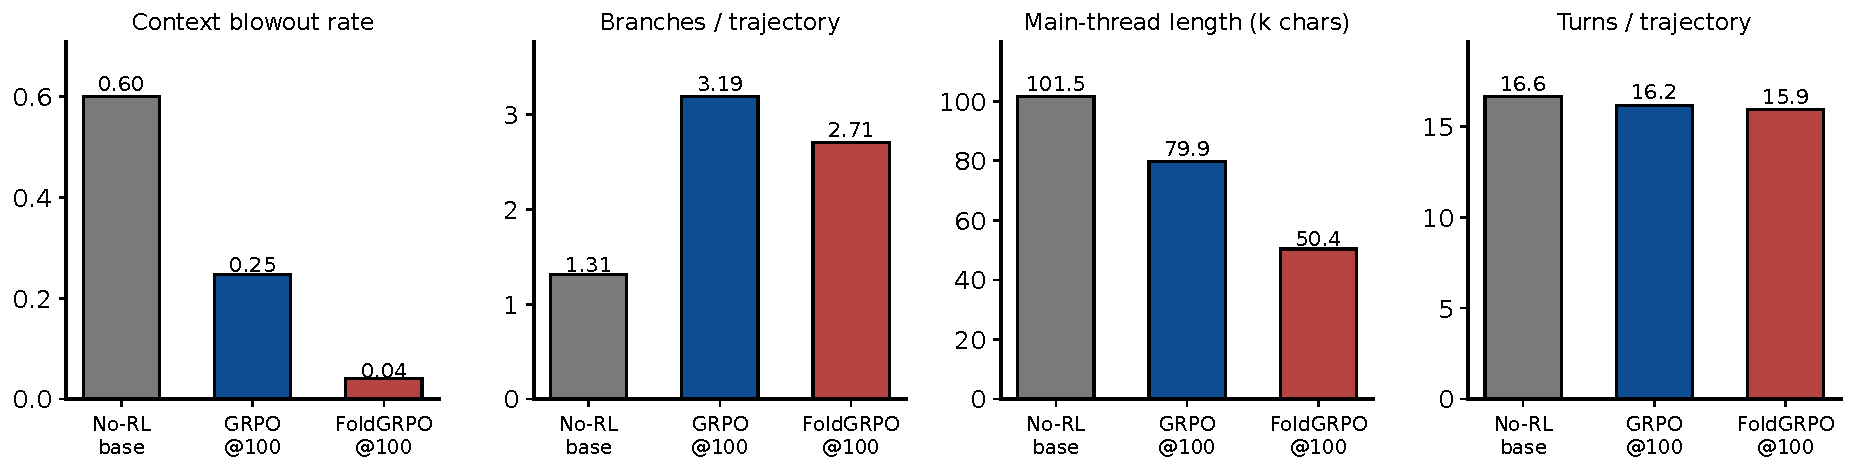
\includegraphics[width=\linewidth]{figures/fig3_behavior_signatures.pdf}
\caption{Behavioral signatures by arm under greedy decoding (150 trajectories per arm):
context-blowout rate, branches per trajectory, and total generated text (the panel label
``main-thread length'' predates this correction; the quantity is full-session characters).}
\label{fig:behavior}
\end{figure}

\begin{figure}[t]
\centering
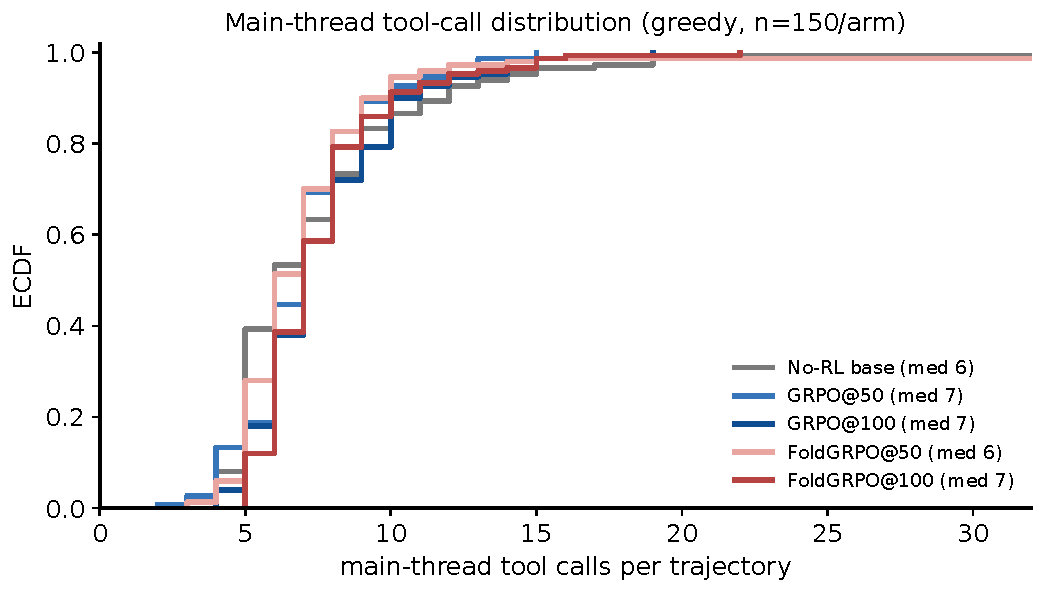
\includegraphics[width=0.85\linewidth]{figures/fig4_turns_ecdf.pdf}
\caption{Empirical CDF of tool calls per trajectory (greedy, $n{=}150$ per arm), counted over
the full generation stream including branch interiors; the in-figure axis label reads
``main-thread'' and predates this correction.}
\label{fig:ecdf}
\end{figure}
